\subsection{Materiali e descrizione}
L'esperimento consiste nel lasciar cadere una sferetta, in questo caso di metallo, all'interno di un fluido e annotare coppie di valori empirici velocità-tempo confrontandoli con quelli teorici ricavati dalla formula trovata nella sezione precedente. Sinceramente non sono molto soddisfatto degli esperimenti fatti perché il tempo di caduta è troppo breve e questo causa un errore grossolano sia sul rilevamento dei tempi che sull'affidabilità dei valori. Il problema è dovuto al fatto che avrei dovuto scegliere una sferetta di raggio minore (ma non ne avevo in casa), questo perché l'attrito del fluido non è solo proporzionale alla velocità della sfera, ma anche al suo raggio; la legge di Stokes completa per una sfera è infatti:
\begin{equation}
    F_s = - 6\pi\mu rv
\end{equation}
mentre la sua forza antagonista, \(F_pf\) è proporzionale al volume che va come \(r^3\) quindi, per \(r\) grandi, la forza peso vince\footnote{\MakeUppercase{è} simile al rapporto che c'è tra superficie e volume delle cellule: il motivo per cui non abbiamo poche cellule grandi ma tante cellule piccole è che gli scambi chimici avvengono sulla superficie e il rapporto tra superficie e volume non può essere troppo piccolo altrimenti la cellula morirebbe. In una sfera (la nostra cellula) \(V \propto R^3\), mentre \(S \propto R^2\) ne segue che \(S/V \propto 1/R\) e quindi se R cresce troppo la cellula non ha sufficienti scambi per poter stare in vita.} e la sferetta cade svelta. Per limitare i danni ho fatto le riprese a rallentatore per aumentare la precisione delle misure.

\begin{wrapfigure}{r}{0.35\textwidth} %this figure will be at the right
    \centering
    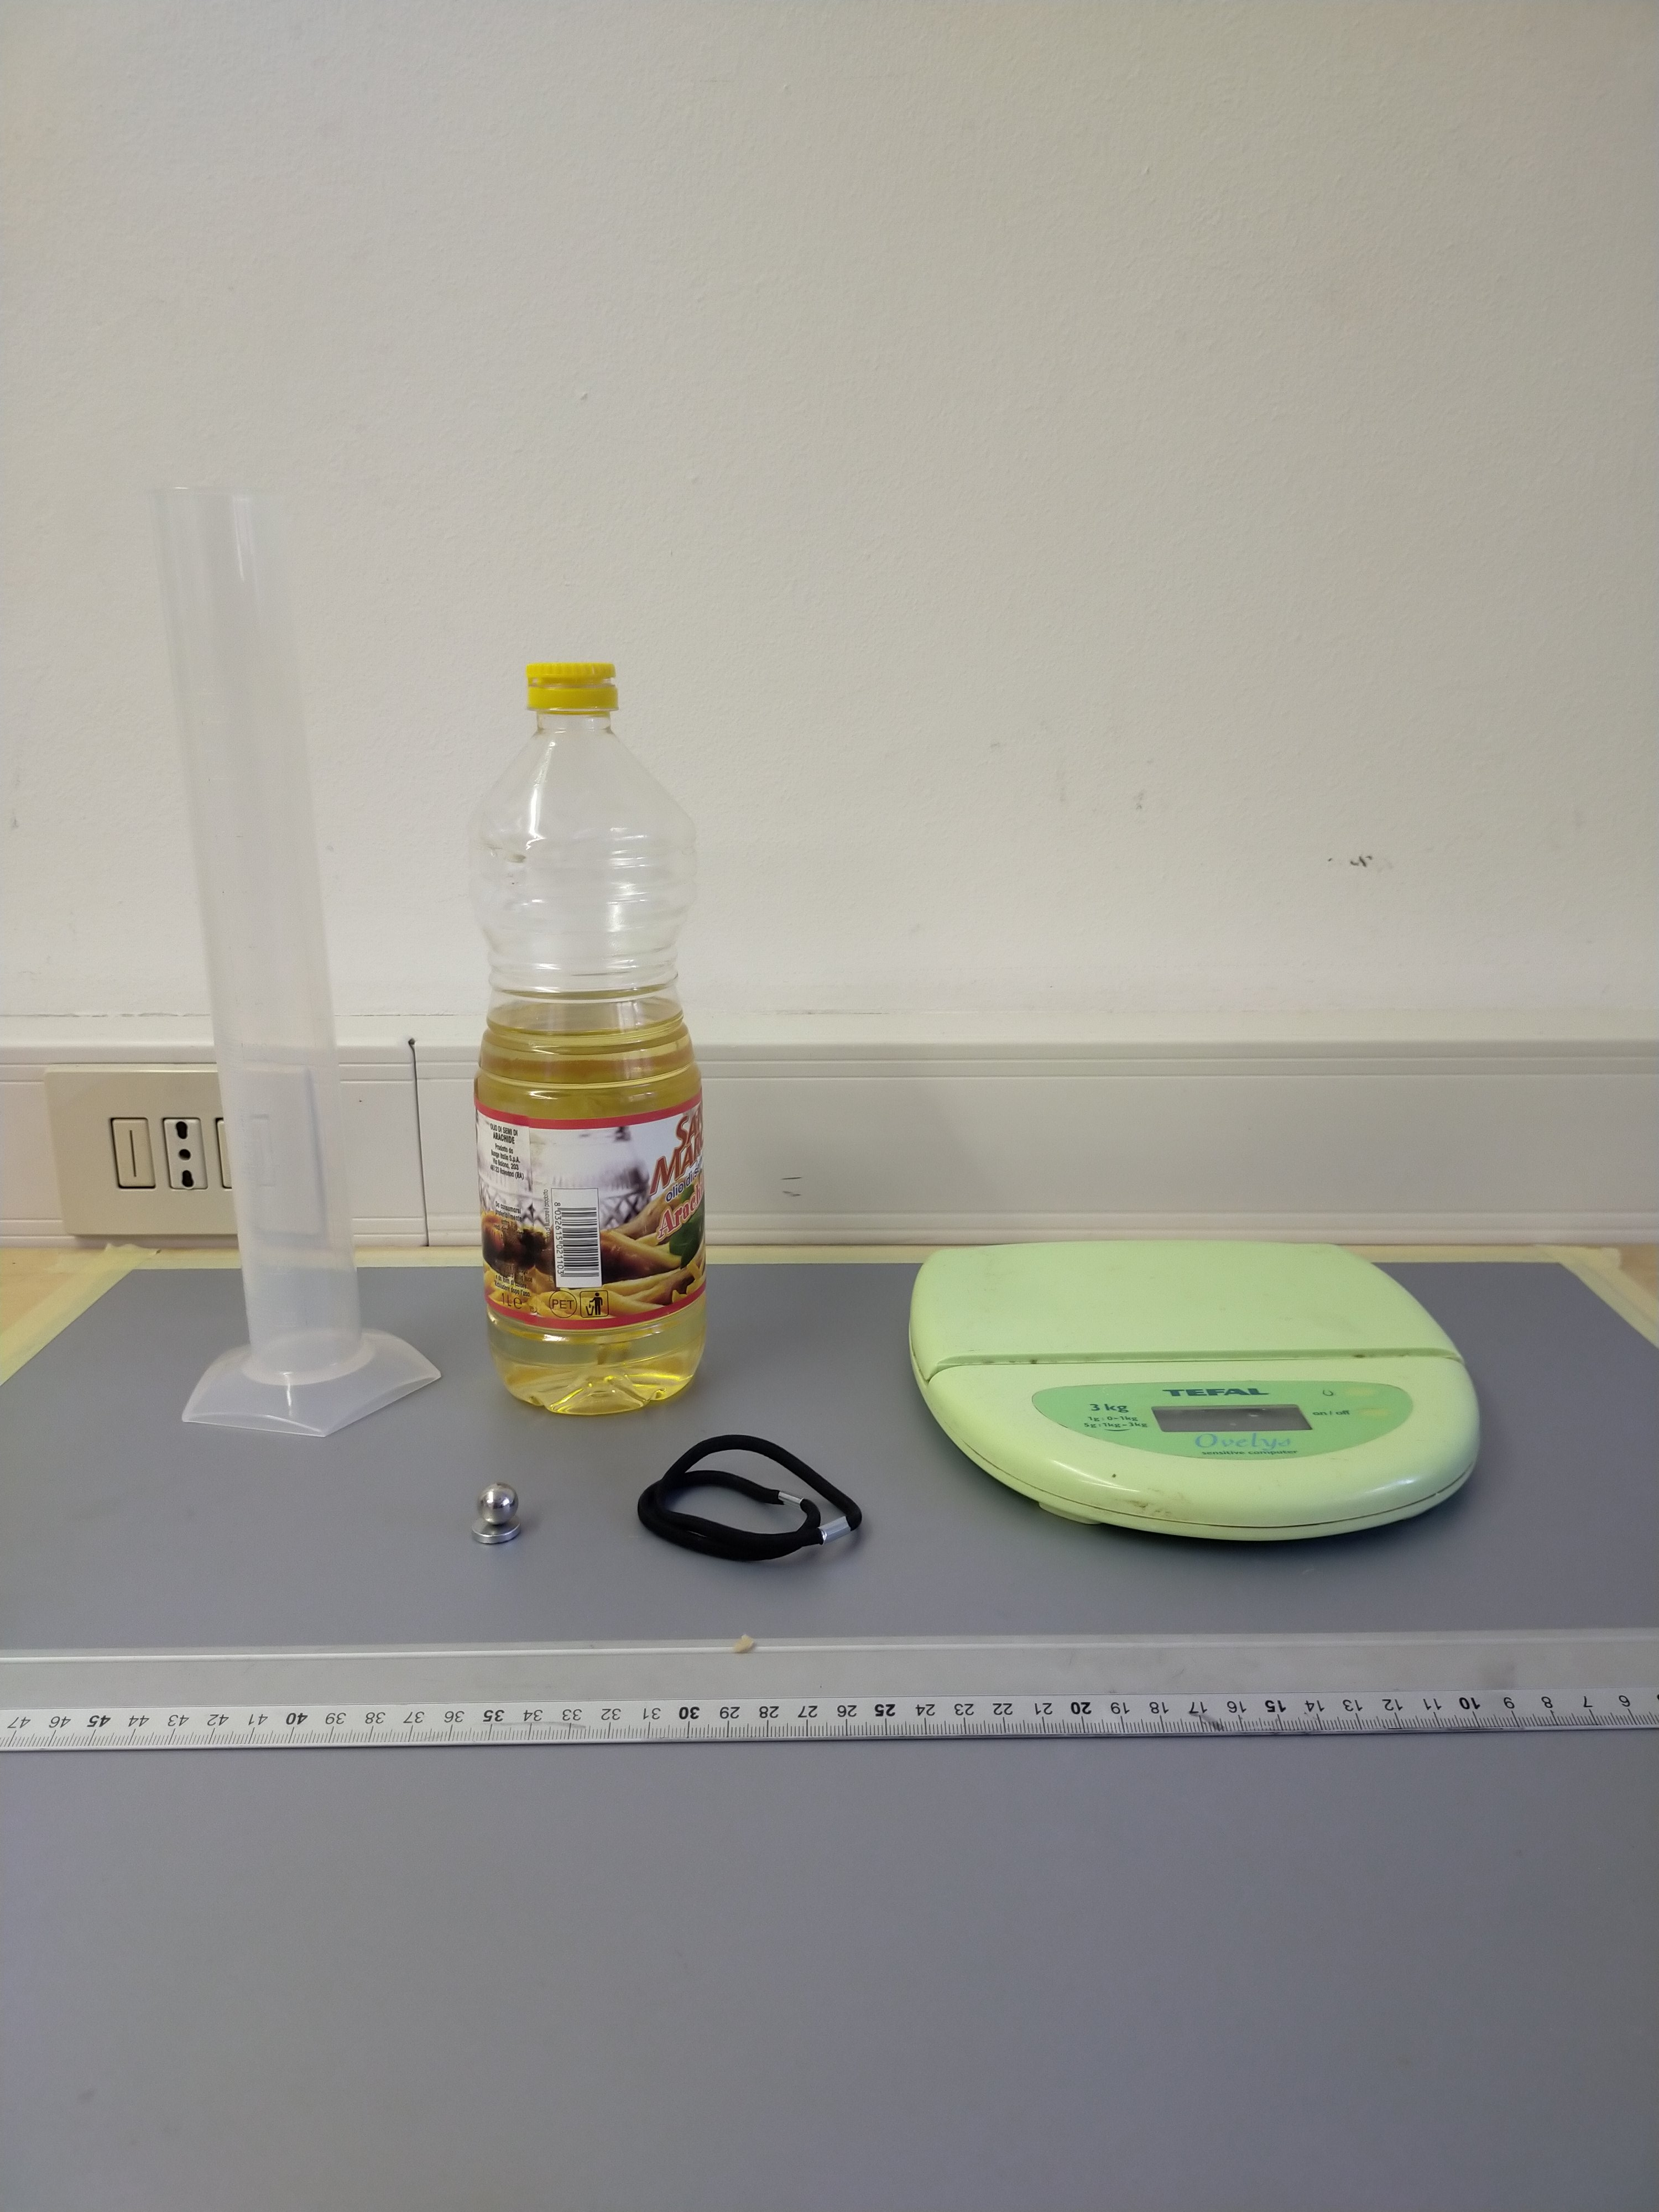
\includegraphics[width=0.35\textwidth]{images/img0.jpg}
    \caption{materiali}
\end{wrapfigure}

\raggedright\textbf{Lista materiali}
\texttt{
\begin{itemize}
    \item Cilindro graduato.
    \item Righello.
    \item Sferetta di metallo.
    \item Olio di semi.
    \item Elastici.
    \item Bilancia.
    \item Magneti (opzionale).
\end{itemize}
}

\clearpage
Un altro problema che ho riscontrato riguarda il timer del telefono che sembra non essere affidabile per quanto riguarda i centesimi di secondo.\\
Per diminuire l'errore sui dati ho deciso, visto gli strumenti digitali a disposizione, di aggiungere alle riprese una barra orrizzontale che ho mappato in modo tale che fosse sempre al centro della mia sfera. 
Supponendo trascurabile la distorsione delle distanze prodotte dall'inclinazione della fotocamera\footnote{Anche se ho avuto cura di posizionare il telefono in modo tale da rendere la normale alla camera più possibile parallela al terreno per limitare questo effetto nulla nella vita è perfetto.} posso utilizzare la posizione in pixel della barra per ricavare una posizione approssimata della sfera nel cilindro. Un ragionamento analogo posso farlo per il tempo: essendo il timer del telefono poco preciso mi affido ai frame del video come unità di misura del tempo. Ovviamente posso poi ricondurmi ad una misura in secondi utilizzando il framerate del video, che è noto, e dando per buoni il $T_{cronometro}$ iniziale e $T_{cronometro}$ finale.
Le equazioni che trasformano $pixel$ in $cm$ e $frame$ in $secondi$ sono le seguenti:
\begin{equation}
s(pxl) = s_0 - \frac{\Delta s}{\Delta pxl}\cdot \delta_{pxl}
\end{equation}
\begin{equation}
t(frame) = t_0 + FPS \cdot \delta_{frame}
\end{equation}
\begin{equation}
\Delta s = \left| s_{finale} - s_{iniziale} \right|
\end{equation}
\begin{equation}
\Delta pxl = \left| pxl_{finale} - pxl_{iniziale} \right|
\end{equation}






